%%%%%%%%%%%%%%%%%%%%%%%%%%%%%%%%%%%%%%%%%%%%%%%%%%%%%%%%%%%%%%%%%%%%%%%%%%%%%%%%%%%%%%%%%%%%%%%%%%%%%
%
%   Version     : 4.0
%
%   Filename    : main.tex
%
%   Description : This is the main file for the LaTeX thesis proposal document template.
%                 The template is intended for use by students under the Department of Software Technology. 
%
%                It is assumed that you can learn how to use LaTeX on your own.
%                Please check/read the following online LaTeX book:
%
%                                 http://en.wikibooks.org/wiki/LaTeX
%     
%   Author      : Florante R. Salvador
%
%   Contributors: 1.  Karlo Campos (former faculty member)
%                 2.  Briane Paul V. Samson 
%   
%   Notes       : Please email the DST Thesis Coordinator, Mr. Edward Tighe (edward.tighe@dlsu.edu.ph), for feedback and suggestions
%
%   Reference:
%
%
%   History/Updates:
%      March 12, 2009:
%           -- created version 1.0 for release to CSC701M (Methods of Research) students
%      May 30, 2009   
%           -- updated Title page and Abstract for undergrad ST students
%      Feb 27, 2015 (version 2)
%           -- changed class to report, created a figures folder, 
%              removed unnecessary packages, added new comments  based on Ethel Ong's slides
%      Feb 24, 2018 (version 3)
%           -- Reorganized the chapters, i.e., Chapter 3 is now Theoretical Framework 
%              and Chapter 4 is now Research Methodology.
%           -- Included the Research Ethics documents as Appendix A.
%      June 15, 2022 (version 4)
%           -- Updated the title page
%           -- Revised text for figures and references
%
%%%%%%%%%%%%%%%%%%%%%%%%%%%%%%%%%%%%%%%%%%%%%%%%%%%%%%%%%%%%%%%%%%%%%%%%%%%%%%%%%%%%%%%%%%%%%%%%%%%%%%

%%%%%%%%%%%%%%%%%%%%%%%%%%%%%%%%%%%%%%%%%%%%%%%%%%%%%%%%%%%%%%%%%%%%%%%%%%%%%%%%%%%%%%%%%%%%%%%%%%%%%%%%%%%%%%%%%%%%%%%
%
%  Filename   : preamble.tex
%
%  Description: Preamble file to :
%               a. specify related packages
%               b. set margins, commands, etc.
%
%  Note       : Edit the margin settings for your own printer
%                  You may add your own commands, environments (it is assumed that you know what you're doing.)
%
%%%%%%%%%%%%%%%%%%%%%%%%%%%%%%%%%%%%%%%%%%%%%%%%%%%%%%%%%%%%%%%%%%%%%%%%%%%%%%%%%%%%%%%%%%%%%%%%%%%%%%%%%%%%%%%%%%%%%%%

%\documentclass[12pt,titlepage,onepage, letterpaper]{article}

\documentclass[12pt,titlepage,onepage,letterpaper]{report}


%
%-- specify related packages
%

%
% \usepackage[utf8x]{inputenc}
%

\usepackage{pdfpages}

\usepackage{apacite}           %-- APA style citation 
                               %-- refer to http://www.ctan.org/tex-archive/biblio/bibtex/contrib/apacite/
\usepackage{natbib}            %-- Natbib package for \citep and other citation commands
%
%  \usepackage{ucs}
%


\usepackage{amsmath}           %-- American Math Society packages
\usepackage{amsfonts}
\usepackage{amssymb}
\usepackage{booktabs}

\usepackage{graphicx}          %-- graphicx package needed for including figures in JPG or PNG format
 
%
%\usepackage{graphics}          %-- graphics related package (this was commented out) use when image is in EPS format
%

\usepackage{verbatim}          %-- this package allows you to have multiple lines of comments by
                               %-- example:
                               %   \begin{comment}
                               %        ...your text here...
                               %   \end{comment}  

\usepackage{color}             %-- allows use of color with text
                               %-- example:  \textcolor{red}{This is the colored text in red.}

\usepackage{url}  %-- allows use of URLs example: \url{https:\ccs1.dlsu.edu.ph}


%
%-- set margins,  you may need to edit this for your own printer
%
\topmargin 0.0in
\oddsidemargin 0.0in
\evensidemargin 0.0in

\voffset 0.0in
\hoffset 0.5625in

\textwidth 5.75in
\textheight 8.5in


\parskip 1em
\parindent 0.25in

\bibliographystyle{apacite}            %-- use APA citation scheme

\hyphenation{ana-lysis know-ledge}     %-- LaTeX may not hyphenate correctly some words you use in your document
                                       %-- use \hyphenation to instruct LaTeX how to do it correctly, example above

\newcommand{\degree}{^{\circ}}         %-- use \newcommand to create your own "commands"
                                       %-- \newcommand works like the #define you learned in your COMPRO1 class

\newcommand{\etal}{et al.}


%\newcommand{\sinag}{\emph{Sinag}}
%\newcommand{\sinagtwo}{\emph{Sinag2}}

\newcommand{\figref}[1]{Figure \ref{#1}}
\newcommand{\appref}[1]{Appendix \ref{#1}}

%-- \newcommand{\Section}[1]{\section{#1}\setcounter{figure}{0}\setcounter{table}{0}}

%\newcommand{\shade}{\multicolumn{1}{|>{\columncolor[gray]{0.25}}c|}{}}
%\newcommand{\tableheader}[1]{\rowcolor{black}\color{white}{#1}}
%\newcommand{\cell}[2]{\multicolumn{1}{#1}{#2}}
%\newcommand{\definition}[2]{\textbf{\textit{#1}} --- #2}
%\newcommand{\itembit}[1]{\item \textbf{\textit{#1}}}
%\newcommand{\sgdef}[2]{\parbox[t][][t]{1.75in}{\textbf{#1}} \> \parbox[t][][t]{4.0in}{#2}\\\\}

%\newenvironment{sinagglossary}{\begin{flushleft}
%\begin{tabbing}
%\hspace{1.75in}\=\\}{\end{tabbing}\end{flushleft}}

\newcommand{\thestitle}[1]{{\Large \textsc{#1}}}


%---
%  \renewcommand{\thefigure}{\thesection.\arabic{figure}}
%  \renewcommand{\thetable}{\thesection.\arabic{table}}
%  \renewcommand{\contentsname}{Table of Contents}

                %-- includes LaTeX source file for the preamble 
                                  %-- include packages, sets the margin sequence, and many more... 
                                  %-- your job: check if the settings are suitable for your own printer

\graphicspath{{figures/}}  %-- figures is the name of the folder containing images JPG or PN

\begin{document}

%%%%%%%%%%%%%%%%%%%%%%%%%%%%%%%%%%%%%%%%%%%%%%%%%%%%%%%%%%%%%%%%%%%%%%%%%%%%%%%%%%%%%%%%%%%%%%%%%%%%%%
%
%   Filename    : title_page.tex 
%
%   Description : This file will contain your Title Page.
%                 
%%%%%%%%%%%%%%%%%%%%%%%%%%%%%%%%%%%%%%%%%%%%%%%%%%%%%%%%%%%%%%%%%%%%%%%%%%%%%%%%%%%%%%%%%%%%%%%%%%%%%%

\begin{titlepage}
\centering


%-- **EDIT** the following line to indicate your thesis title. Try to keep it within 20 words for brevity, and focus on highlighting the intended contribution of your work.
\thestitle{A Multimodal Approach on Automatic Personality Recognition of Filipino Instagram Users}

\vspace{1.5cm}

A Thesis Proposal\\

\vspace{0.5cm}

presented to\\

\vspace{0.5cm}

the Department of Software Technology\\
College of Computer Studies\\
De La Salle University

\vspace{1cm}

In partial fulfillment\\
of the requirements for the degree of\\

\vspace{0.5cm}

%Master of Science in Computer Science
Bachelor of Science in Computer Science\\
Major in Software Technology
\vspace{1.75cm}
\\by\\


%% EDIT the following line to indicate the complete names of all your group members arranged in alphabetical order 
\vspace{1cm}

Chen, Ting Rung  \\
De Veyra, Rebecca  \\
Giron, John Joseph  \\
Rodriguez, Joaquin Andres D.  \\

\vspace{1.75cm}
%-- **EDIT** the following line to indicate your adviser's name 
Edward Tighe \\
Adviser

\vspace{1.75cm}
\today
\end{titlepage}
              %-- includes LaTeX source file for the Title Page 
                                  %-- your job: **EDIT THIS FILE ** to indicate your own title, name, and thesis adviser's name


%%%%%%%%%%%%%%%%%%%%%%%%%%%%%%%%%%%%%%%%%%%%%%%%%%%%%%%%%%%%%%%%%%%%%%%%%%%%%%%%%%%%%%%%%%%%%%%%%%%%%%%
%
%   Filename    : abstract.tex 
%
%   Description : This file will contain your abstract.
%                 
%%%%%%%%%%%%%%%%%%%%%%%%%%%%%%%%%%%%%%%%%%%%%%%%%%%%%%%%%%%%%%%%%%%%%%%%%%%%%%%%%%%%%%%%%%%%%%%%%%%%%%

\begin{abstract}
\begin{mdframed} [style=highlight]
Filipino Automatic Personality Recognition (APR) has predominantly focused on using Twitter from the PagkataoKo dataset using only text features from tweets. While Filipino Instagram users represent a rich source of behavioral data, no current APR research leverages both image and text modalities for this demographic, despite evidence that visual and linguistic cues jointly enhance trait prediction. To address this, we propose the first multimodal APR framework for Filipino Instagram users, combining VGG-19-derived image features with bilingual (English/Tagalog) text analysis to advance beyond unimodal approaches. Our classification methodology employs SVM and XGBoost models with intermediate attention-based fusion of image-text-metadata features, systematically comparing unimodal and multimodal performance across Big Five traits while adhering to ethical guidelines established in the PagkataoKo Dataset.  
\end{mdframed}




%
%  Do not put citations or quotes in the abract.
%
\end{abstract}
                %-- this is the Abstract page
                                  %-- your job: **EDIT THIS FILE** to indicate your own abstract
%%%%%%%%%%%%%%%%%%%%%%%%%%%%%%%%%%%%%%%%%%%%%%%%%%%%%%%%%%%%%%%%%%%%%%%%%%%%%%%%%%%%%%%%%%%%%%%%%%%%%%
%
%   Filename    : abstract.tex 
%
%   Description : This file will contain your abstract.
%                 
%%%%%%%%%%%%%%%%%%%%%%%%%%%%%%%%%%%%%%%%%%%%%%%%%%%%%%%%%%%%%%%%%%%%%%%%%%%%%%%%%%%%%%%%%%%%%%%%%%%%%%

\begin{abstract}
\begin{mdframed} [style=highlight]
Filipino Automatic Personality Recognition (APR) has predominantly focused on using Twitter from the PagkataoKo dataset using only text features from tweets. While Filipino Instagram users represent a rich source of behavioral data, no current APR research leverages both image and text modalities for this demographic, despite evidence that visual and linguistic cues jointly enhance trait prediction. To address this, we propose the first multimodal APR framework for Filipino Instagram users, combining VGG-19-derived image features with bilingual (English/Tagalog) text analysis to advance beyond unimodal approaches. Our classification methodology employs SVM and XGBoost models with intermediate attention-based fusion of image-text-metadata features, systematically comparing unimodal and multimodal performance across Big Five traits while adhering to ethical guidelines established in the PagkataoKo Dataset.  
\end{mdframed}




%
%  Do not put citations or quotes in the abract.
%
\end{abstract}

\pagenumbering{roman}             %-- this will number pages as i, ii, iii, etc...
\setcounter{page}{2}

\tableofcontents                  %-- this command is used to generate the Table of Contents


\newpage
\listoffigures                    %-- this command is used to generate List of Figures

\newpage                       
\listoftables                     %-- this command is used to generate List of Tables

\newpage

\pagenumbering{arabic}            %-- this will number pages as 1, 2, 3, etc...
\setcounter{page}{1}              


%%%%%%%%%%%%%%%%%%%%%%%%%%%%%%%%%%%%%%%%%%%%%%%%%%%%%%%%%%%%%%%%%%%%%%%%%%%%%%%%%%%%%%%%%%%%%%%%%%%%%%
%
%   Filename    : chapter_1.tex 
%
%   Description : This file will contain your Research Description.
%                 
%%%%%%%%%%%%%%%%%%%%%%%%%%%%%%%%%%%%%%%%%%%%%%%%%%%%%%%%%%%%%%%%%%%%%%%%%%%%%%%%%%%%%%%%%%%%%%%%%%%%%%

\chapter{Introduction}
\label{sec:intro}    %--note: labels help you with hyperlink editing (using your IDE)

Social media platforms have been used as means of self-expression for users. These platforms give users the possibility to express and expose their identity \citep{Marcus2006}. As such, data from social media platforms can lead us to gain insights from personality traits of these users. 

%%This chapter builds the motivation for the conduct of the research through a description of the background of the study or the current state of technology. This is followed by the research objectives, the scope and limitations, and significance of the research. The chapter ends with the research methodology describing the different activities to be conducted to achieve the goals of this research.%%


%%
%% --- 1.1 Background of the Study --- %%
%%

\section{Background of the Study}
\label{sec:overview}

%
%   NOTE: You have to delete/replace the unnecessary paragraphs with your own text.
%


%%This section gives the reader an overview of the specific technology or field in the international or local setting. The information regarding the technology or field should be contemporary and not
%%based on outdated sources. Discussion must not be too technical or too detailed.

%%Follow the inverted pyramid to describe each of the following. Allocate one (1) paragraph per level in the pyramid. 

% Describe the research area
%Research area ...

This study's main research area is on personality computing. Personality computing is related to artificial intelligence and personality psychology by studying one's personality through a variety of computational techniques from different sources (usually text, multimedia, and social networks). Among the three main problems personality computing addresses; automatic personality recognition, perception, and synthesis \citep[p.~280]{Vinciarelli2014}; this study focuses on automatic personality recognition.


% Describe the domain (where will you apply the topic)

Automatic personality recognition (APR) aims to infer the personality of an individual based on their digital footprint. APR has been traced back to the work of \citet{Pennebaker1999} wherein they asked the question of \textit{can language use reflect personality style?}


% Give a synthesis of previous work

% Synthesis of previous studies...
\citet{Pennebaker1999} and \citet{Mairesse2007} had demonstrated the different ways of detecting personalities and emotions by analyzing the text with various language models. Due to that, social media had became a common place for the research of personality detection. The PagkataoKo dataset has been made with social media activity on Instagram and X (formerly known as Twitter). There were more studies using X's data than Instagram due to X being a more prominent platform with its text-based posts. However, \citet{ferwerda2016}, \cite{Reece2017-qw} and \cite{Harris2019-gq} made studies that showed analyzing photos was possible. Thus, researching on Instagram became more meaningful in this manner.


% State the problem and the research question

% Paragraph containing the Problem Statement or the Research Question.

After looking over the research, a gap when it comes to using image data in personality recognition was identified. Given this, the study aims to further explore approaches for implementing APR using social media data, specifically Instagram. The study aims to address the question: How can Instagram content, including images and captions, be used to infer a Filipino’s personality traits based on psychological and computational analysis?

% This section ends with a discussion on the problem/s faced by or that still exist in the specific technology or field (e.g., limitations of existing software or algorithms). It should not contain your research objectives or goal; instead, the problem statement would lead to the research objectives to be stated in 1.2.

% \subsection{Figures}

% Often times, a graph, illustration, screenshot, or any image can help a reader better understand what we say in text. In academic writing, we call them \textbf{figures}. Please add as many figures as necessary to help build your narrative, but do not go overboard. 

% You can add figures in JPG or PNG format as shown in Figure \ref{fig:disneystock}. All figures should also have a descriptive caption. As a general principle, your caption should adequately describe what is shown in the figure, and not just short texts. If we remove all the surrounding text, the reader should still understand what your figure is. 

% All figures should be referred to at least once in the surrounding paragraphs. Make sure that you explain what the figure is all about, and that you refer to your figure. You can also use the surround paragraphs to highlight key insights or parts of your figure. For example, \figref{fig:disneystock} shows a graph of the performance of Disney stock from the 1980s to 2012.

% %--- the following example shows how to include a figure in PNG format
% \begin{figure}[t]                %-- use [t] to place figure at top, [b] to place at the bottom, [h] for here
%    \centering                    %-- use this to center the figure
%    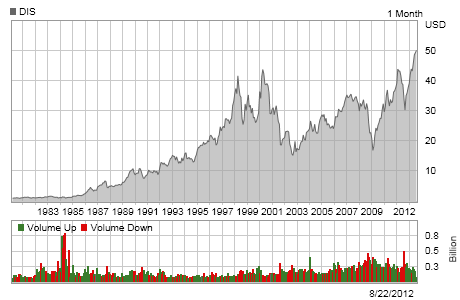
\includegraphics{DisneyChart.png}      %-- include image file named as "disneychart.png" 
%    \caption{Disney's stock price chart from the 1980s up to 2012. The top chart shows the stock price in each month. The bottom chart shows the change in volume of transactions. The bars are colored based on the type of movement that happened in a month.}
%     \label{fig:disneystock}
% \end{figure}

% \subsection{References}

% Some notes on citing references. When using APA format, the author-date method of citation is followed. This means that the author's last name and the year of publication for the source should appear in the text, and a complete reference should appear in the reference list.

% %
% % Examples:
% %     	Smith (1970) compared reaction times . . .
% %     	In a recent study of reaction times (Smith, 1970), . . .   
% %     	In 1970, Smith compared reaction times . . .
% %	Smith, et al., (1970) compared reaction times . . .
% %     	In a recent study of reaction times (Smith, et al., 1970), . . .  
% %     	In 1970, Smith, et al., compared reaction times . . .
% %

% Here are some examples on how to do the referencing (note author's name and years are different from commented examples). For APA citation details, refer
% to \url{http://www.ctan.org/tex-archive/biblio/bibtex/contrib/apacite/}. 

% \begin{itemize}
%  \item \citeA{kartch:2000:ERA} compared reaction times...
%  \item In a recent study of reaction times \cite{kartch:2000:ERA}...
%  \item In \citeyearNP{kartch:2000:ERA}, \citeauthor{kartch:2000:ERA} compared reaction times...
%  \item \shortciteA{fedkiw:2001:VSO} compared reaction times... 
%  \item In a recent study of reaction times \cite{fedkiw:2001:VSO}...
%  \item In \citeyearNP{fedkiw:2001:VSO}, \shortciteauthor{fedkiw:2001:VSO}, compared reaction times...
% \end{itemize}

% The following are references from journal articles \cite{Park:2006:DSI, Pellacini:2005:LAH, sako:2001:SSB}.  Here's an MS thesis document \cite{yee:2000:SSA}, and this is from a PhD dissertation \cite{kartch:2000:ERA}. For a book, reference is given as \cite{parke:1996:CFA}.  Proceedings from a conference samples are \cite{Jobs95, fedkiw:2001:VSO,levoy:2000:TDM}.  

% The sample bibliography file named \textbf{myreferences.bib} is from the
% SIGGRAPH \LaTeX template.  You can use a text editor to view the contents of the bib file. It is your task to create your own bibliography file.  For those who downloaded papers from ACM or IEEE sites, there is a BibTeX link that you can click; thereafter, you just simply need to copy and paste the BibTeX entry into your own bibliography file.

% \subsection{Code snippet}

% The following shows how to include a program source code (or algorithm). The verbatim environment, as the name suggests, outputs text (including white spaces) as is...

% \begin{verbatim}
%                #include <stdio.h>
%                main()
%                {
%                     printf("Hello world!\n");
%                }
% \end{verbatim}


%%
%% --- 1.2 Research Objectives --- %%
%%

% \section{Research Objectives}

% This subsection states the over--all goal that must be achieved to answer the problem. Address the following: Given your research challenge or opportunity, how do you intend to solve it? What is the main outcome of your research? What kind of contribution do you want to achieve?

% The \textbf{general objective} is broken down into three or more specific objectives. The \textbf{specific objectives} are relatively smaller objectives that help you attain your general objective. You can formulate your specific objectives based on your running questions about the project. For example, the group does not have a good picture yet of the different conversation patterns between humans that can be mimicked by conversational agents. A specific objective can be "to identify different human-human conversation patterns." These objectives must be specific, measurable, attainable, realistic, and time-bounded.

% Reviewing related literature, studying a particular programming language or development tool (e.g., to study Windows/Object-Oriented/Graphics/C++ programming), and documentation to accomplish the general objective is inherent in all thesis projects and, therefore, must not be included here.


\begin{comment}
%
% IPR acknowledgement: the following sentences and examples are from Ethel Ong's slides 
%     on Research Objectives
%

How to formulate your research objectives:
1. Identify what research steps do you need to perform to achieve your general objective.
2. Identify the questions that must be answered for you to achieve your general objective.
    Thereafter, convert these questions into action statements


Example #1:

Question:
    What strategies do human educators employ in collaborative storytelling with children?

Specific Objective:
   To review existing strategies employed by language educators when sharing storytelling with children


Example #2:

Question:
   How will you represent commonsense knowledge for use by computer systems?

Specific Objective:
   To identify knowledge representation approaches used by existing story generation systems

Example #3:
Question:
   What types of storytelling knowledge are needed to generate stories?

Objective:
    To identify the different types of storytelling knowledge used in generating stories

Example #4:
Question:
    What machine learning approaches will you utilize?

Specific Objective:
    To determine existing machine learning algorithms [that can be used in training the computer system to detect cyberbullying cases] 

Example #5: 
Question:
    How will your research output be evaluated?

Specific Objective:
    To define evaluation metrics for validating the accuracy of the translation
\end{comment}


%
%  The following is the format for presenting your specific objectives; replace them with your own 
%

% The specific objectives of this research are as follows:
% \begin{enumerate}
%    \item To identify knowledge representation approaches used by existing story generation systems;
%    \item To identify the different types of storytelling knowledge used in generating stories;
%    \item To build a neural-based model for generating events comprising a story; and
%    \item To define evaluation metrics for evaluating the performance of the event generation model.
% \end{enumerate}


%%
%% --- 1.3 Scope and Limitations --- %%
%%

% \section{Scope and Limitations of the Research}
% \label{sec:scopelimitations}

% This section discusses the boundaries, with respect to the objectives, of the research and the constraints within which the research will be developed. Describe what is and is not included in the scope of your research, supported by your main research question and findings of previous studies. Do not use weak excuses such as the lack of time and/or knowledge to perform the research.

% A good rule of thumb is to allocate one paragraph for each of your specific objectives that (1) contains a brief overview of the concept/theory and the purpose of doing the associated objective; and (2) includes a description of the scope/limitation of your study, and followed by brief purpose, rationale and/or justification for your decisions.

% The following should also be indicated in your Scope and Limitations (in the appropriate paragraphs matching the objectives, or as a stand-alone paragraph):
% \begin{itemize}
%    \item The profile and demographics of your target participants
%    \item Your data sources (i.e., new data, data from previous studies, data to be provided by some experts, data to be retrieved from social networks)
%    \item The specific technology platform to be utilized
%    \item The methods for collecting the data
%    \item The coverage areas or locations
%    \item The duration or time period (e.g., news articles for the year 2016-2017)
% \end{itemize}


%%
%% --- 1.4 Significance of the Research --- %%
%%

\section{Significance of the Research}
\label{sec: Significance}

To our knowledge, image features in Filipino APR have not been explored yet. Therefore, exploring this would maybe give better insights on how images from Filipino Instagram Users tell their personality.  While existing studies have largely focused on textual data from platforms like Twitter, our study expands the scope by incorporating visual elements from Instagram and fusing these two features: textual data and image data. 

This study also addresses the underrepresentation of Filipino social media data in personality recognition research. By utilizing data in both English and Filipino languages alongside visual content, this research displays whether there is a significant improvement in predicting the personality of Filipinos when integrating image features as well. Moreover, this study investigates whether combining text and image features results in a significant improvement in personality prediction accuracy compared to unimodal approaches. 

Apart from benefiting Filipino APR research, this study possibly benefits marketing, advertising, and social networking platforms as well. In \cite{Matz2017} study on Psychological Targeting in Digital Marketing, it was found that by aligning ad content with the personality traits of target audiences, marketers can enhance engagement and conversion rates (the percentage of users who take a desired action after being exposed to a targeted advertisement). 

%%This section explains why research must be done in this area.  It rationalizes the objective of the research with that of the stated problem. Avoid including sentences such as ``This research will be beneficial to the proponent/department/college'' as this is already an inherent requirement of all BS and MS thesis projects.  Focus on the research's contribution to the Computer Science field.

%%The following are guide questions that may help your formulate the significance of your research. 


%
% IPR acknowledgement: the following list of items are from Ethel Ong's slides on Significance of the Research
%
%%\begin{itemize}
%%\item  What is the relevance and contribution of your work to the computer science community? 

%%\begin{itemize} 
%%\item How does your technical contributions or empirical findings advance the field or grow our body of knowledge? 
%%\item If you built a prototype of an interaction technique, interface, library, tool, or system, what is value does it add compared to existing solutions? 
%%\end{itemize}

%%\item What will be your contributions to society in general? 
%%    \begin{itemize}
%%      \item How will your main stakeholders benefit from your technical contributions or empirical findings? 
%%      \item What are the positive social or economic impacts? 
%%%%   \end{itemize}
%%\end{itemize}

\begin{comment}
If applicable, describe possible commercialization and/or innovation in your research.
\end{comment}               %-- includes LaTeX source file for Chapter 1: Research Description
                                  %-- your job: **EDIT THIS FILE** to indicate your own research description

%%%%%%%%%%%%%%%%%%%%%%%%%%%%%%%%%%%%%%%%%%%%%%%%%%%%%%%%%%%%%%%%%%%%%%%%%%%%%%%%%%%%%%%%%%%%%%%%%%%%%%
%
%   Filename    : chapter_2.tex 
%
%   Description : This file will contain your review of related works.
%                 
%%%%%%%%%%%%%%%%%%%%%%%%%%%%%%%%%%%%%%%%%%%%%%%%%%%%%%%%%%%%%%%%%%%%%%%%%%%%%%%%%%%%%%%%%%%%%%%%%%%%%%

\chapter{Related Works}
\label{sec:Related Works}

\section {Single Modal Approaches to APR}
\label{sec: SMApproaches}

\section{Multimodal Approaches to APR}
\label{sec: MMApproaches}
The earliest multimodal APR studies primarily focused on audio and visual features extracted from recorded conversations and behavioral interactions. \citet{Pianesi2008} conducted a study on multimodal behavioral analysis in multi-party meetings, utilizing SVM classifiers to predict Big Five personality traits and Locus of Control based on speech and facial expressions. Their results showed that facial features contributed significantly to extraversion classification, while vocal features were more informative for conscientiousness.

Following this, \citet{Sidorov2014} employed a similar audio-visual approach using data from the SEMAINE dataset, which consists of emotionally colored conversations. The study evaluated different segmentation techniques to improve classification accuracy, concluding that shorter segments provided better performance for certain personality traits.

Expanding on audio-visual models, \citet{Lima2022} introduced a deep learning approach, incorporating text data alongside audio and visual cues. Their research used Recurrent Neural Networks (RNNs) to process sequential multimodal data, extracting temporal dependencies in social interactions. Their model was trained on 9.1 million parameters, demonstrating the scalability and computational complexity of deep learning-based APR systems.

As social media platforms became a dominant mode of communication, researchers shifted towards analyzing text and image data to infer personality traits. \citet{Machajdik2010} introduced an affective image classification model, which extracted color, texture, and composition-based features to predict emotional responses. Although not directly designed for personality classification, their findings laid the foundation for future studies connecting visual aesthetics with personality traits.

\citet{Xianyu2016} extended this approach by introducing a heterogeneity-entropy-based deep learning framework that combined text, images, and social media interactions. Their model used Deep Belief Networks (DBNs) and Autoencoders to extract latent personality features, highlighting how unsupervised learning techniques can capture subtle personality cues across modalities.

\citet{Skowron2016} further refined multimodal approaches by integrating linguistic, visual, and metadata features from Twitter and Instagram. Their study incorporated LIWC for linguistic analysis and emotion detection techniques from Machajdik and Hanbury (2010) to extract visual features. Their findings demonstrated that cross-platform personality modeling improved accuracy, emphasizing that personality traits manifest differently across different social networks.

Advancements in machine learning-based personality prediction have allowed researchers to refine image and text-based multimodal models for social media applications. \citet{Ferwerda2018} developed a personality recognition model based on Instagram images, utilizing the Google Vision API for image content extraction and a ZeroR classifier for baseline evaluation. Their results indicated that image aesthetics and content types strongly correlate with personality traits, particularly in openness and extraversion classification.

Similarly, \citet{Batrinca2016} examined multimodal cues in team-based interactions, incorporating speech, body movements, and facial expressions to model collaborative personality traits. Their study used Hidden Markov Models (HMMs) and SVMs, demonstrating that nonverbal behavior plays a significant role in personality assessments within group settings.

\citet{Branz2020} refined the image-based personality recognition model by analyzing color preferences in Instagram photos. Their study confirmed that specific color choices (e.g., dominant red hues) correlated with openness, while blue hues were linked to conscientiousness. The study utilized k-Nearest Neighbors (k-NN) and SVMs, establishing a connection between color psychology and personality traits in digital environments.

The latest advancements in multimodal APR have shifted toward deep learning-based models, with an emphasis on personalization and adaptive AI techniques. \citet{Salam2022} introduced a personalized personality prediction model, utilizing Neural Architecture Search (NAS) to optimize Deep Neural Networks (DNNs) for different user demographics. Their study found that customized models outperformed generic APR models, reinforcing the importance of personalization in AI-driven personality recognition.

Building on deep learning methodologies, \citet{Lima2022} leveraged sequential data modeling to improve real-time personality prediction. Their model incorporated Long Short-Term Memory (LSTM) networks, demonstrating that capturing temporal dependencies enhances classification accuracy. Their research concluded that personality traits are not static but evolve based on user interactions, emphasizing the potential of adaptive AI-driven personality assessments.

\section{Learning Approaches to APR}
\label{sec: LearningApproaches}

\section{Filipino APR}
\label{sec: FilipinoAPR}

%Previous draft
%\citet{Pennebaker1999} explored on their study how language use can reflect the personality style of someone. Using a computerized word-based text analysis program, the structure, validity, and reliability of the written language was examined. From there it was found that one's linguistic style is a consequential way to explore personality.

%This was further explored in a study by \citet{Mairesse2007} in which the recognition of the Big Five Personality traits (Openness, Conscientiousness, Extroversion, Agreeableness, and Neuroticism) on both text and conversation was first experimented using both self rating and observer ratings of personality. From the experimentation done with the various models: classification, ranking, and regression; the ranking models performed best overall.

%The PagkataoKo dataset analyzed in this paper has been used in the studies of undergraduates, graduates, and professionals at DLSU. These various studies primarily involved modeling Filipino users’ personality traits or Automatic Personality Recognition (APR) through their usage of the Instagram and X (formerly Twitter) social media sites, as was the purpose of the creation of the dataset. 

%The dataset contains data on Filipino social media users’ social media activity on Instagram and Twitter. This includes features like post images and captions,  profile pictures, follower and following counts, and post count. It also includes the user’s BFI scores.

%Among the undergraduate and graduate studies that pursued the analysis of this dataset, the majority of them utilized only the X data, focusing on natural language processing. Techniques such as word embedding models, topic modeling, feature extraction, and other models were used to predict the BFI personality traits of users. One used both X and Instagram, but only the text data was used. There also exists another study that analyzed the visual features of Instagram image data and used this to predict personality traits. Lastly, a published study also used text processing on the X data for the same purpose.

%X was a more popular choice for analysis as the platform's main focus is that it is more text-based and the captions hold the most importance whereas on Instagram, it is more secondary. This leaves the Instagram portion of the dataset relatively unexplored compared to the X data, so there is little information about image processing in this dataset. However, this leaves open the potential for exploring images and their relation to personality, specifically the BFI scores, adding to the one research that was done on this topic. 

%Filipinos use social media in many ways. They use it for connecting with other people, sharing information, speaking out, and optimizing productivity \citep{10.1007/978-3-031-61543-6_24}. However, even though they are aware of the presence of social media, \citet{Cruz_Jamias_2013} found that Filipino researchers rarely use social media to their advantage. This demonstrates that each demographic in the Philippines has a different level of social media use.

%Social media has many effects in the Philippines. For instance, it plays a role in youth political participation. \citet{Ibardeloza2022-pz} found that social media helps the youth to be more exposed to radical involvement. It also has a positive effect on “peer interpersonal relationships” yet slightly negative on familial relationships \citep{Bristol2016TheDM}.

%Recent studies have explored the potential of Instagram image data to infer users' personality traits. \citet{ferwerda2016} analyzed features such as hue, brightness, and saturation in users' photos, finding significant correlations between these visual elements and the Big Five personality traits. Their findings suggest that individuals' choices in photo appearance can reflect underlying personality characteristics. 

%Further research by \citet{Reece2017-qw} utilized machine learning to examine Instagram photos for markers of depression. By analyzing color properties, metadata, and the presence of faces, their model successfully identified depressive indicators, highlighting the platform's potential for mental health screening. 

%Additionally, a study by \citet{Harris2019-gq} investigated the accuracy of personality portrayal on Instagram by comparing observers' perceptions of account holders' personalities with the account holders' self-reported traits. The results indicated discrepancies, suggesting that while certain visual cues can convey personality aspects, they may also lead to misinterpretations. 

%Collectively, these studies underscore the viability of leveraging Instagram image data to assess users' personality traits and mental health status, though they also caution against overreliance on visual cues due to potential misrepresentations.


%%This chapter provides a synthesis of past research, existing algorithms, and or state-of-the-art software that are related/similar to the thesis. It should not present detailed summaries of each related work, but rather present a cohesive comparison of different aspects of their work. At the end of each section and this chapter, it should be clear what research challenges and opportunities will be focused on for the proposal.

%%The sections can be about approaches, application areas, and categories of solutions that give readers an deep understanding of the current state of the field. 

%%Observe a consistent format when presenting each of the reviewed works. This must be selected in consultation with the prospective adviser.

%%\textcolor{red}{DO NOT FORGET to cite your references.} Related works can be discussed multiple times in different sections of this chapter, depending on what is being discussed or compared.


\begin{comment}
%
% IPR acknowledgement: the contents within this comment are from Ethel Ong's slides on RRL.
%
Guide on Writing your Related Works chapter
 
1. Identify the keywords with respect to your research
      One keyword = One document section
                Examples: 2.1 Story Generation Systems
			 2.2 Knowledge Representation

2.  Find references using these keywords

3.  For each of the references that you find,
        Check: Is it relevant to your research?
        Use their references to find more relevant works.

4. Identify a set of criteria for comparison.
       It will serve as a guide to help you focus on what to look for

5. Write a summary focusing on -
       What: A short description of the work
       How: A summary of the approach it utilized
       Findings: If applicable, provide the results
        Why: Relevance to your work

6. At the end of each section,  show a Table of Comparison of the related works 
   and your proposed project/system

\end{comment}
















               %-- includes LaTeX source file for Chapter 2: Review of Related Literature
                                  %-- your job: **EDIT THIS FILE** to indicate your review of related literature 

%%%%%%%%%%%%%%%%%%%%%%%%%%%%%%%%%%%%%%%%%%%%%%%%%%%%%%%%%%%%%%%%%%%%%%%%%%%%%%%%%%%%%%%%%%%%%%%%%%%%%%%
%
%   Filename    : chapter_3.tex 
%
%   Description : This file will contain your Theoretical Framework.
%                 
%%%%%%%%%%%%%%%%%%%%%%%%%%%%%%%%%%%%%%%%%%%%%%%%%%%%%%%%%%%%%%%%%%%%%%%%%%%%%%%%%%%%%%%%%%%%%%%%%%%%%%

\chapter{Theoretical Framework}
\label{sec:theoframework}
Please refer to the following resources regarding Theoretical Framework: 

\begin{itemize}

\item \url{https://link.springer.com/chapter/10.1007/978-1-4419-1454-5_12}
\item \url{https://link.springer.com/article/10.1007/s10972-015-9443-2}



\end{itemize}


               %-- includes LaTeX source file for Chapter 3: Theoretical Framework
                                  %-- your job: **EDIT THIS FILE** to indicate your research methodology

%\chapter{Methodology}
\label{sec:methodology}

This chapter enumerates and discusses the specific steps and activities that will be performed by the proponent to accomplish the objectives of the research. The discussion covers the activities from pre-proposal to Final Thesis Writing. 

Ethical issues surrounding the research and the steps to be taken by the research team to adhere to ethical guidelines and principles should be included when discussing each of the activities.

Research activities include inquiry, survey, research, brainstorming, canvassing, consultation, review, interview, observe, experiment, design, test, document, and other similar tasks. The following sections present an example set of activities and methods for conducting computing research. \textbf{\textcolor{red}{However, note that your group's actual research activities and methods will be different depending on your intended research contributions. You should consult closely with your thesis adviser for proper guidance. The following sections need not appear in your actual thesis proposal.}}

\section{Data Collection}

This section, also called "Data Gathering", focus on activities that will enable the researchers to understand their users and their context better, or to analyze the operating environment where the proposed software may be deployed. The types of activities would include interviews, observations, surveys, focus group discussions, and review of secondary data (reports, videos, manuals) to enable the researchers to identify user requirements; learn the existing processes, strategies, rules and guidelines; and/or build the datasets and knowledge resources needed in the study.

Ethical issues surrounding the collection of data from human participants, and from internet or 3rd party sources should be indicated. The steps to be taken by the proponents to ensure that ethical guidelines are followed should also be explained.

\section{Software Design and Implementation}

This section covers the design of data structures, knowledge bases, user interface, and algorithms. It includes implementation and related activities - tool selection, unit testing, integration testing, and function testing - that were covered in the course "Software Engineering".

Your Adviser may ask you to separate the Design and the Implementation sections as needed. 

You may also indicate a specific software development lifecycle model that you plan to adopt in developing your software, such as the Agile methodology.

For machine learning types of research, this section may be replaced with "Model Training".

\section{Validation}

This section contains the different types of validation activities that you will conduct to evaluate the performance of your model or algorithm or software. It may include user perception studies, end user acceptance testing, usability test, and model validation.

Ethical issues surrounding the collection of data from human participants should be indicated. The steps to be taken by the proponents to ensure that ethical guidelines are followed should also be explained.

This section should include a discussion of the following if working with human participants:
\begin{itemize}
    \item Participant Selection. Who are your target participants? How will they be selected? What data will be collected?
    \item Orientation. How will ethics be observed? What documents, e.g., validation protocol, will be shared with participants to orient them regarding the research and the validation procedure? Will there be an Informed Consent and Informed Assent? Are they found in the Appendix? Will there be any pre-tests or interviews to be administered prior to the actual experiment?
    \item Experiment Proper (aka Procedure). How long is the experiment or how long should the user use your software? Is it one-on-one, or one-to-many? What will you do while the experiment is ongoing - observe the participants using a checklist, guide the participants, record the interaction/usage?
    \item Debriefing. After the experiment, will you administer any post-tests or debriefing to solicit feedback from your participants? What are these?
\end{itemize}

\subsection{Calendar of Activities}

For the proposal, a Gantt chart showing the schedule of the activities should be added. You can create a table like below, or create a figure. For example:

Table \ref{tab:timetableactivities} shows a Gantt chart of the activities.  Each bullet represents approximately one week worth of activity.

\begin{table}[]
    \centering
    \begin{tabular}{l|c|c|c|c|c|c|c|c|c}
         \toprule
         & \multicolumn{6}{c|}{2021} & \multicolumn{3}{c}{2022} \\
         \textbf{Activity} & \textbf{Apr} & \textbf{May} & \textbf{Jun} & \textbf{Jul} & \textbf{Aug} & \textbf{Sep} & \textbf{Jan} & \textbf{Feb} & \textbf{Mar} \\
         \midrule
         Data Collection & **** & **** & & & & & & & \\
         \midrule
         Software Design & & **** & **** & **** & **** & **** & & & \\
         \midrule
         Validation & & & & & & **** & **** & **** & \\
         \bottomrule
    \end{tabular}
    \caption{Gantt Chart of Activities}
    \label{tab:timetableactivities}
\end{table}               %-- includes LaTeX source file for Chapter 4: Research Methodology
                                  %-- your job: **EDIT THIS FILE** to indicate your research methodology

\appendix                         %-- used to specify appendices
%%%%%%%%%%%%%%%%%%%%%%%%%%%%%%%%%%%%%%%%%%%%%%%%%%%%%%%%%%%%%%%%%%%%%%%%%%%%%%%%%%%%%%%%%%%%%%%%%%%%%%%
%
%   Filename    : appendix_A.tex 
%
%   Description : This file is for including the Research Ethics Documents (delegated as Appendix A) 
%                 
%%%%%%%%%%%%%%%%%%%%%%%%%%%%%%%%%%%%%%%%%%%%%%%%%%%%%%%%%%%%%%%%%%%%%%%%%%%%%%%%%%%%%%%%%%%%%%%%%%%%%%

\chapter{Research Ethics Documents}
\label{sec:appendixa}


\begin{comment}

IMPORTANT -- READ THIS PART!!!

Please follow the instructions below on how to include the Research Ethics documents 
in your proposal document (typeset using LaTeX):

1. Open, and accomplish the contents of the THREE Word DOCX files included in the distribution

2. Once you're done filling in the necessary items, save the file in PDF format.  This is done by clicking on "File", 
    then "Save As" and then choose PDF (not DOCX default option) .  Do this for the three documents.

   The filenames are long, so I renamed the files with shorter names: 
       a . clearance.PDF  (original was GradSchool-revised ethics clearance form)
       b. general_checklist.PDF (original was General Research Ethics Checklist)
       c.  checklist-A PDF (original was [Specific Checklists] Checklist A - Human Participants]

\end{comment}


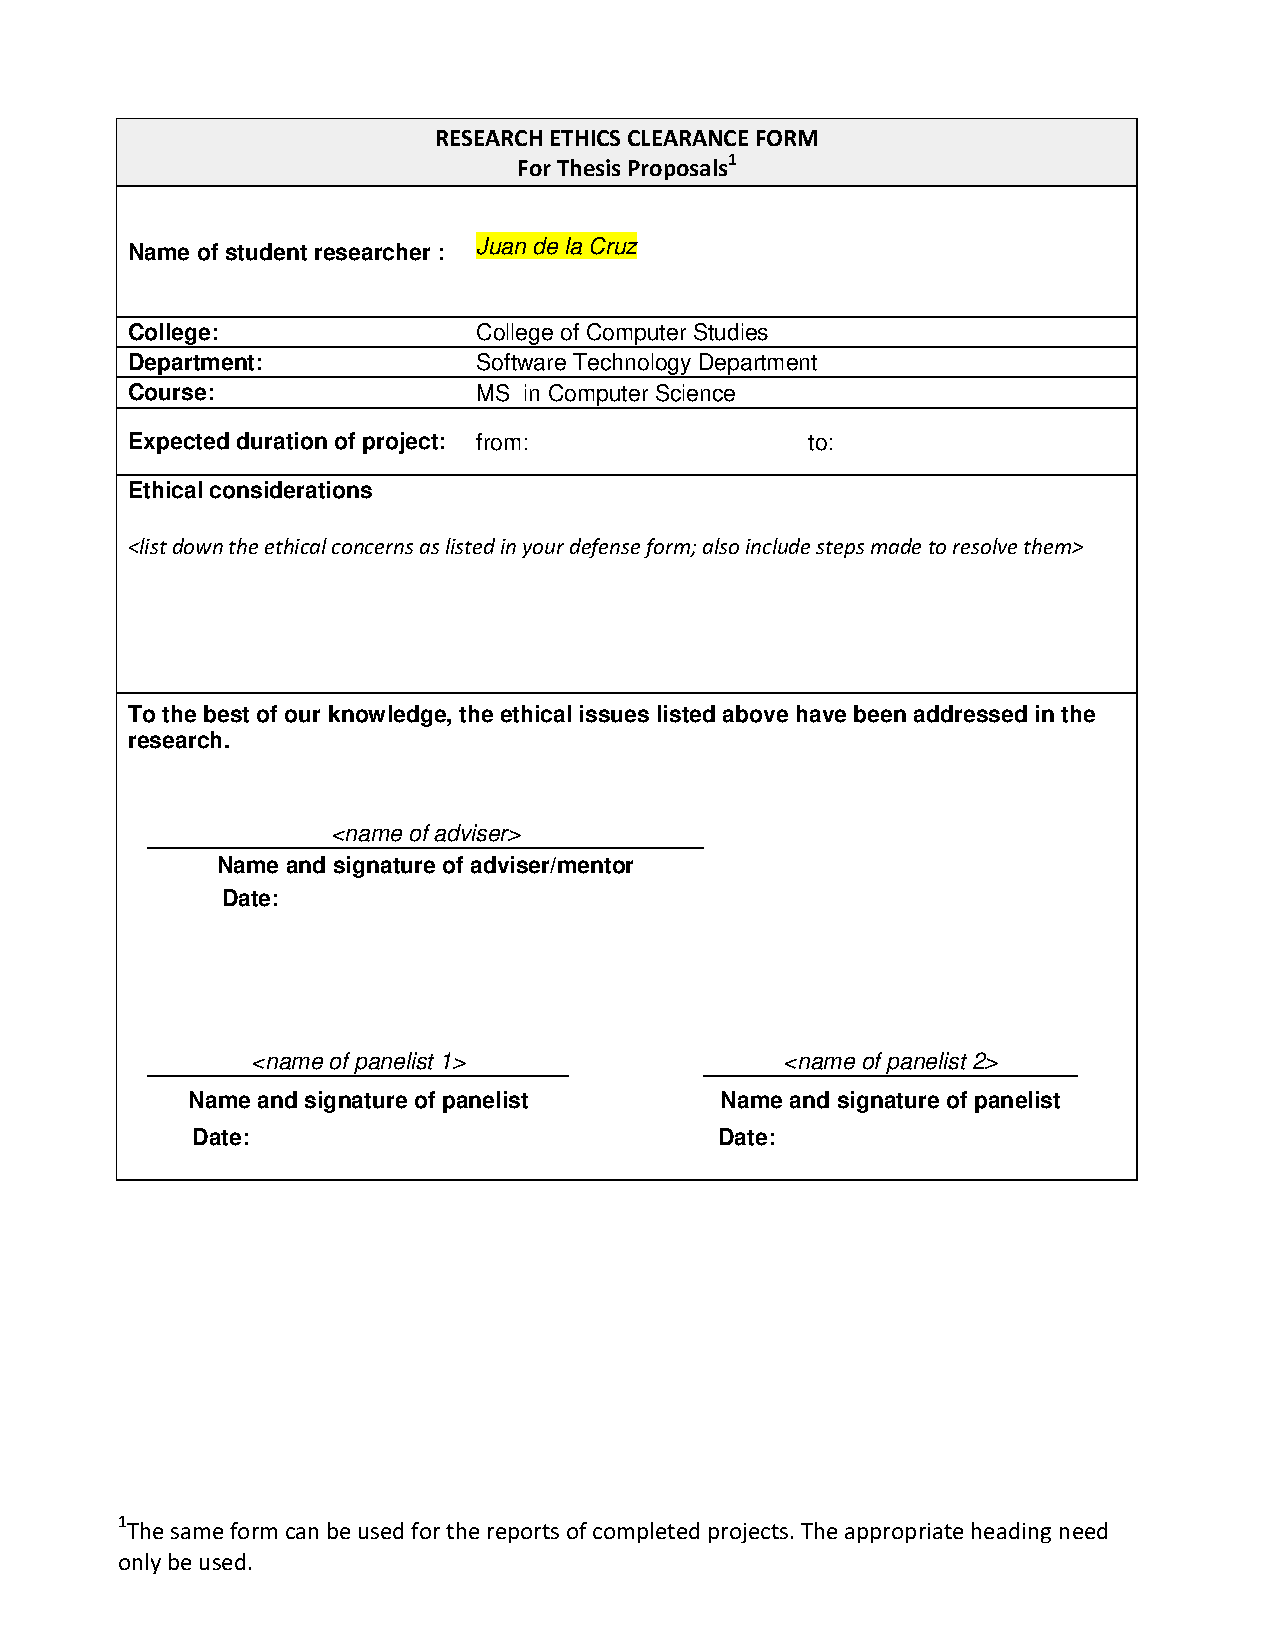
\includepdf[pages=-, scale = 0.9, pagecommand={}, offset = -30 0]{clearance.pdf}

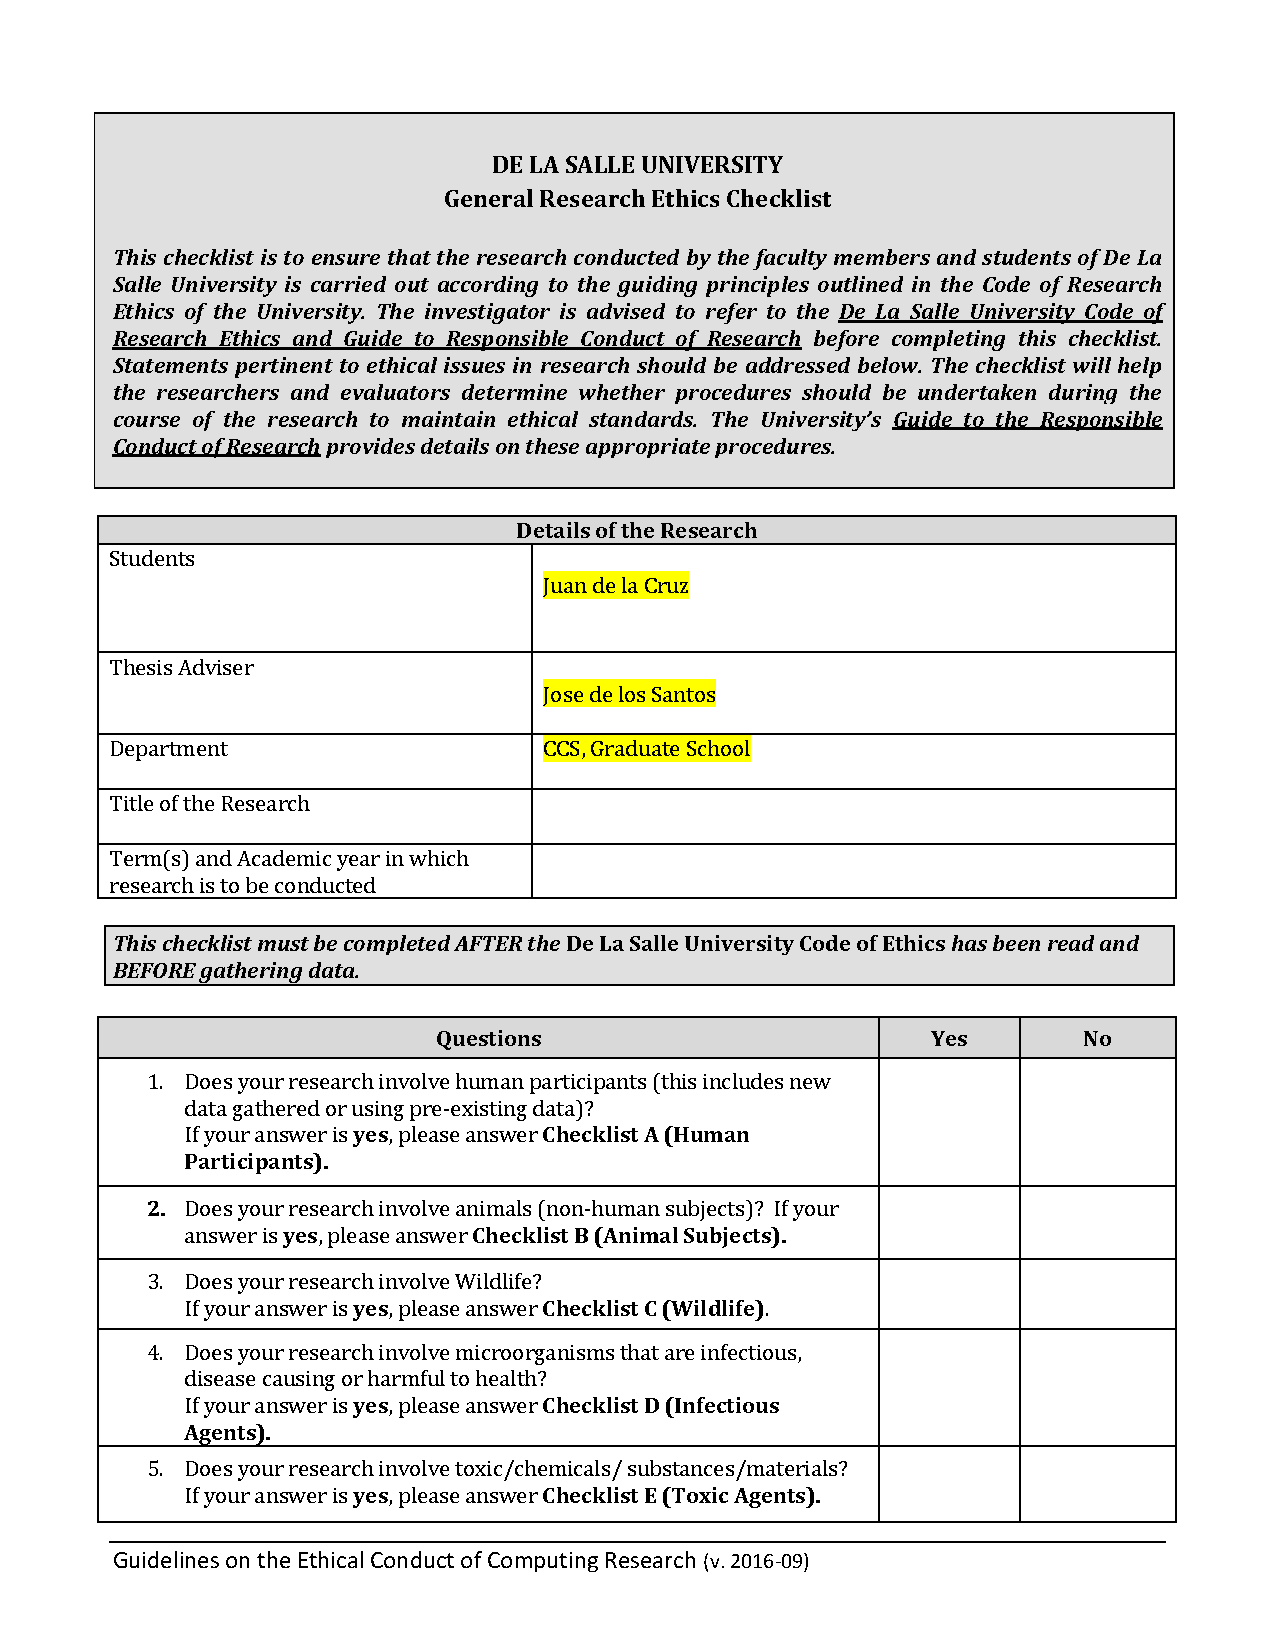
\includepdf[pages=-, scale = 0.9, pagecommand={}, offset = -30 0]{general_checklist.pdf}

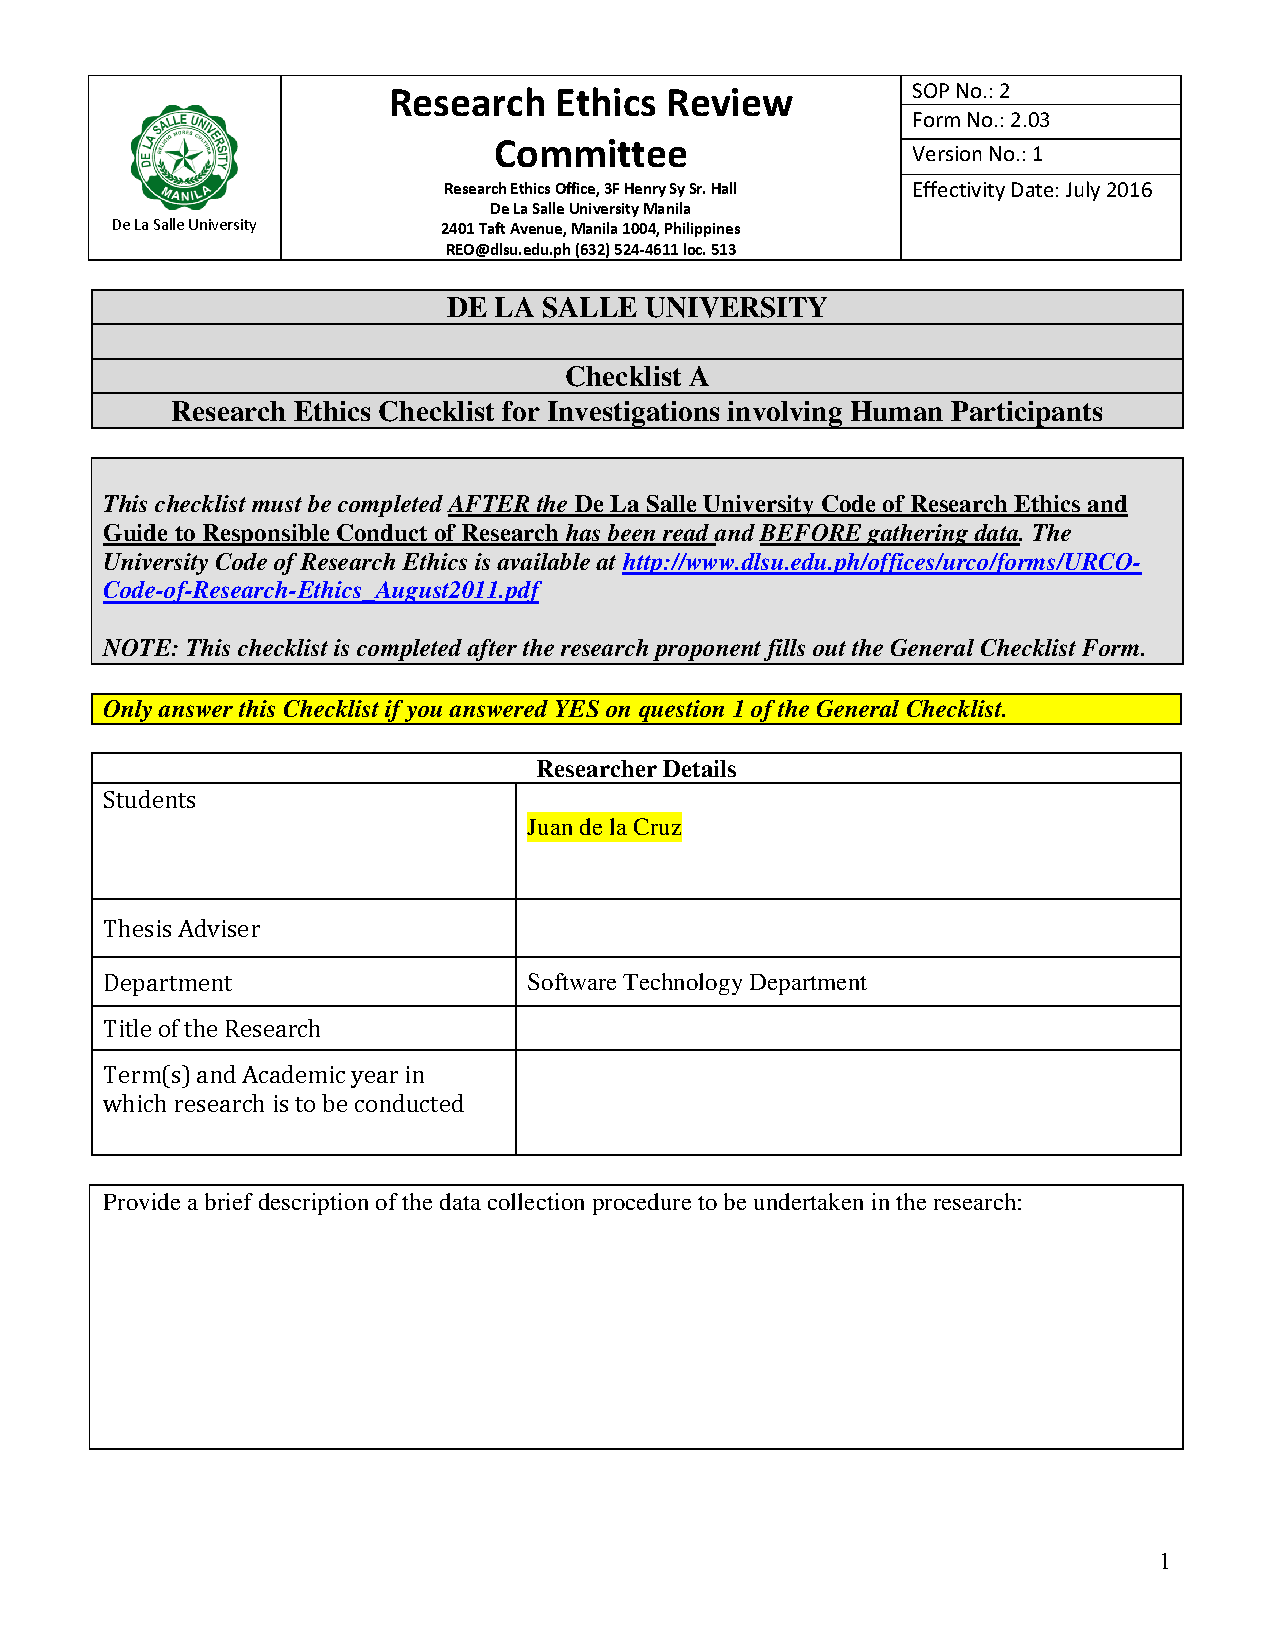
\includepdf[pages=-, scale = 0.9, pagecommand={}, offset = -30 0]{checklist-A.pdf}


              %-- includes LaTeX source file for Appendix A
                                  %-- your job: **CREATE/EDIT** your own source file for the appendices
%%%%%%%%%%%%%%%%%%%%%%%%%%%%%%%%%%%%%%%%%%%%%%%%%%%%%%%%%%%%%%%%%%%%%%%%%%%%%%%%%%%%%%%%%%%%%%%%%%%%%%%
%
%   Filename    : appendix_B.tex
%
%   Description : This file will contain information about your Resource Persons
%                 
%%%%%%%%%%%%%%%%%%%%%%%%%%%%%%%%%%%%%%%%%%%%%%%%%%%%%%%%%%%%%%%%%%%%%%%%%%%%%%%%%%%%%%%%%%%%%%%%%%%%%%

\chapter{Resource Persons}
\label{sec:appendixc}

%
%  Indicate your resource persons here:
%
%	<full name and title, e.g., Dr. Juan de la Cruz>
%	<profession, e.g., faculty>
%	<department, e.g., College of Computer Studies>
%	<name of institution, e.g., De La Salle University>
%	<e-mail address>
%
%

%
%  the following shows 3 examples, replace entries with your own
%
\newcommand{\resperson}[4]{\textbf{#1} \\ #2 \\ #3 \\ \url{#4}\vspace{0.5em}\\}

\resperson{Dr. Firstname1 Lastname1}{Adviser}{College of Computer Studies\\De La Salle University-Manila}{emailaddr@dlsu.edu.ph}
\resperson{Mr. Firstname2 Lastname2}{Role2}{Affiliation2}{emailaddr2@domain.com}
\resperson{Ms. Firstname3 Lastname3}{Role3}{Affiliation3}{emailaddr3@domain.net}




%\bibliographystyle{apacite}       %-- specified APA style for bibliograpy
                                  %-- more details about APA style citation can be found in www.ctan.org/tex-archive/biblio/bibtex/contrib/apacite/

                                  %-- bibliographic entries are handled via bibtex; refer to www.bibtex.org for more details


\bibliography{myreferences}       %-- the file "myreferences.bib" is a sample bibliography (bib) from SIGGRAPH 
                                  %-- your job: **CREATE/EDIT** your own bibliography file  

\end{document}

